\documentclass[a4paper,
DIV=13,
12pt,
BCOR=10mm,
department=FakEI,
%lucida,
%KeepRoman,
%twoside,
parskip=half,
automark,
%headsepline,
]{article}


\usepackage[utf8]{inputenc}
\usepackage{tabularx}
%\usepackage[english]{babel}
\usepackage[ngerman]{babel}
\setlength{\parindent}{0pt}
\date{\today}
\usepackage[table]{xcolor}
\usepackage{graphicx}
\usepackage{abstract}



\title{Stimmungsampel}

\author{Luzia Pfeilschifter und Felix Maier}



%\studentid{123456789 und 3124819}
%\department{Elektro- und Informationstechnik}
%\studyprogramme{Bachelor Elektro- und Informationstechnik}
%\startingdate{1.\,November 2088}
%\closingdate{11.\,Dezember 2089}			%%muss noch geändert werden

%\firstadvisor{Prof. Dr. Paula Streng}
%\secondadvisor{Prof. Dr. Petra Hart}
%\externaladvisor{Dr. Klara Endlos}

%\externallogo[height=1.5cm]{firmenlogo}

\begin{document}
\maketitle
\cleardoublepage
\begin{abstract}
Das Ziel des Projektes war es ein minimalistisches Gerät mit dem STM32G031-Microcontroller zu entwickeln, welches die Stimmung des Trägers mithilfe von LED's darstellt und dabei party-tauglich ist. 

Aus diesem Vorgaben ist das entwickelte Gerät entstanden. Es wird mit einer Knopfzelle betrieben und lässt sich durch eine Berührung mit dem Finger an der Vorderseite des Gehäuses zyklisch, wie eine normale Ampel, weiter schalten. Dies wird durch einen kapazitiven Sensor ermöglicht. Außerdem ist noch ein Schalter verbaut, der die \glqq Stimmung\grqq{} einrasten lässt um beispielsweise ein versehentliches Weiterschalten beim Tanzen zu verhindern. Zudem ermöglicht dieser Schalter eine Reduktion des Stromverbrauchs, wodurch der Partyspaß noch länger anhält.
\end{abstract}
\cleardoublepage
\tableofcontents

\cleardoublepage
\section{Funktionsweise}

Die Funktionsweise werden durch die Abbildung \ref{fig:Register1} und \ref{fig:Register2} dargestellt. 

\begin{figure}[!hbpt]
 \begin{center} 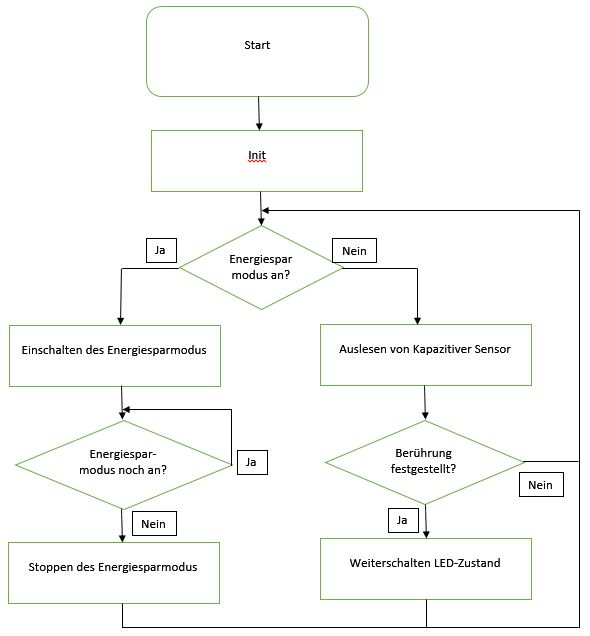
\includegraphics[width=1.1\textwidth]{AblaufMain.jpg}
 \caption{Flussdiagramm zum Ablauf des Hauptprogramms}
 \label{fig:Register1}
  \end{center}
\end{figure}

\begin{figure}[!hbpt]
 \begin{center} 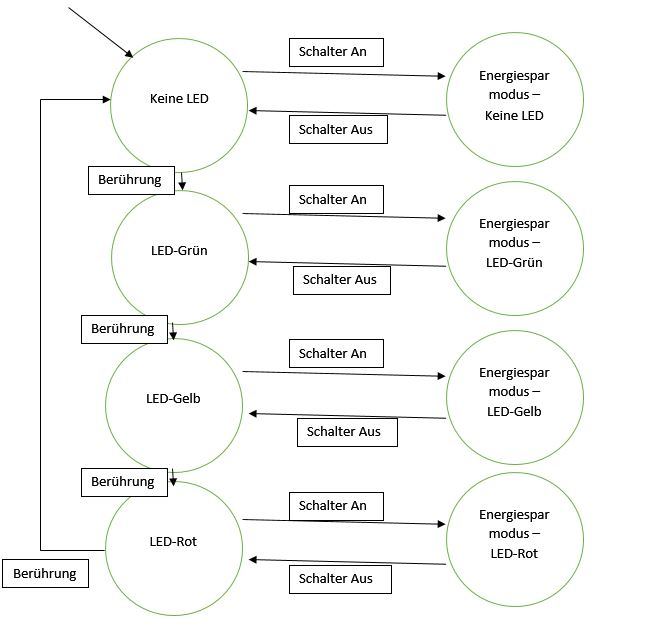
\includegraphics[width=1.1\textwidth]{Zustandsdiagramm.jpg}
 \caption{Zustandsdiagramm}
 \label{fig:Register2}
  \end{center}
\end{figure}



\newpage
\section{Microcontroller}

\begin{figure}[!hbpt]
 \begin{center} 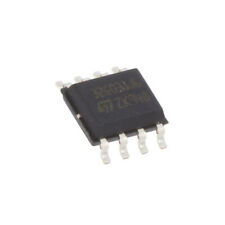
\includegraphics[width=0.3\textwidth]{s-l225.jpg}
 \caption{STM32G031J6M6 als SMD-Baustein QUELLE}
 \label{fig:SMD-Baustein}
  \end{center}

Das Projekt wurde mit dem STM32G031J6M6 (Abbildung \ref{fig:SMD-Baustein}) umgesetzt. Dies ist ein 8-Pin Microcontroller  mit einer ARM 32-Bit Cortex–M0+ CPU, der sehr wenig Strom verbraucht und damit perfekt für diesen Einsatzbereich ist. Er kann mit 1.7 V bis 3.6 V betreiben werden, was gut für die Versorgung mit eine Knopfzelle ist. 

Zudem verfügt er über 4 Oszillatoren, einen DMA-controller, einen ADC, 11 Timer und verschiedene Kommunikationsinterfaces, was völlig ausreichend für dieses Projekt ist QUELLE. 

Dieser Mikrocontroller hat aber auch Nachteile: Einerseits die Pin-Knappheit, da nur 6 Pins programmiert werden können, was die Komplexität der Außenbeschaltungen einschränkt. Die Pinbelegung zeigt hierbei Abbildung \ref{fig:Pinbelegung}.

Andererseits kann es schwer sein diesen Microcontroller zu debuggen bzw. zu flashen, da die Pins 7 und 8 umprogrammiert werden können und somit nicht mehr für der Debug- bzw. Flashvorgang zur Verfügung stehen. Dieses Problem wurde mithilfe des Programmes STM32 ST-LINK Utility, welches eine \glqq Connect under Reset\grqq{}-Option besitzt, gelöst. Dabei wird der Controller in den Reset-Zustand gebraucht. Beim Austreten aus diesen Zustand verbindet es sich mit dem Mikrocontroller bevor der bereits bestehende Code ausgeführt wird, was es erlaubt den Baustein neu zu programmieren.

   \begin{center} 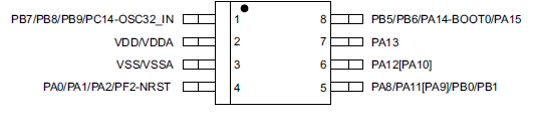
\includegraphics[width=1\textwidth]{Stm32g031j6m6.png}
 \caption{Pinbelegung des Mikrocontrollers STM32G031J6M6 QUELLE}
 \label{fig:Pinbelegung}
  \end{center}  
\end{figure}


\newpage
\section{LED}
\subsection{WS2812b}

Als nächstes wird die Möglichkeit betrachtet eine WS2812b-LED zu verwenden. Sie hat von allen bisherigen LED's die größte Variation an Farben, die dargestellt werden können. Die Ansteuerung erfolgt außerdem nur über eine Datenverbindung, was bei einem Mikrocontroller mit nur 8 Pins sehr vorteilhaft ist.

Die verschiedenen Übertragungsbit können dabei als PWM-Signale mit unterschiedlichen Duty-Cycle aufgefasst werden. So hat eine logische \glqq 0\grqq{} ein Duty-Cycle von 32\% und eine logische \glqq 1\grqq{} ein Duty-Cycle von 68\%. 

Daraus können GRB-Werte gebildet werden, welche durch ein Duty\-Cycle von 0\% über mindestens 50 $\mu$s von den LED's übernommen werden. Dieser komplette Vorgang ist sehr aufwändig für den Prozessor. Deshalb wird der im Mikrocontroller eingebaute DMA-Controller, was für \glqq Direct Memory Access\grqq{} steht, verwendet, um die Auslastung des Prozessors signifikant zu verbessern. 

Die WS2812b LED hat aber insgesamt zwei große Nachteile, die sie schlechter als andere Varianten macht. Zum einen die hohen Kosten, was mit dem Ziel einen möglichst preiswerten Aufbau zu entwerfen kollidiert. Und zum anderen benötigt sie Spannungsversorgung von 5 V, was einen Hochsetzsteller erfordern würde, da der komplette Aufbau mit einer Knopfzelle betrieben wird.

\newpage

\subsection{LED-Schaltung}
\begin{figure}[!hbpt]
 \begin{center} 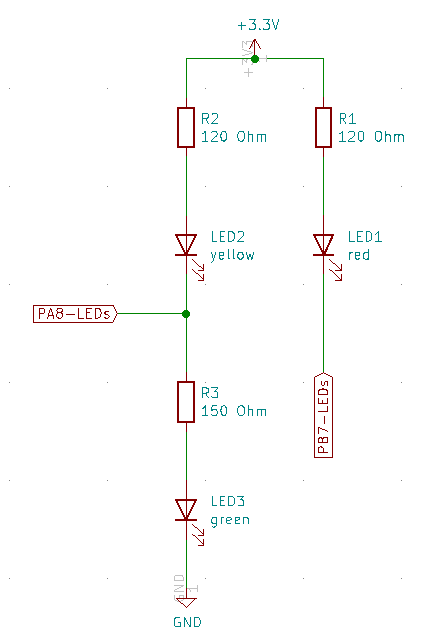
\includegraphics[width=0.7\textwidth]{LED_Schaltung.png}
 \caption{LED Schaltung}
 \label{fig:Register}
  \end{center}
\end{figure}

Letztendlich war eine Schaltung, die mit möglichst wenig Pins möglichst viele LED's ansteuert am sinnvollsten. Um dies zu ermöglichen wurde eine Schaltung entworfen, die mit Hilfe von Input und Output die LED's steuert. 

Dabei können bis zu 4 LED's mit 2 Pins angesteuert werden. In der vorliegenden Ampelschaltung sind nur 3 LED's notwendig, allerdings könnte die 4. noch zwischen Ground und LED1 gehängt werden, wie parallel dazu LED3. Also gibt es 4 verschiedene Zustände, die im folgenden erklärt werden:

\subsubsection{keine LED leuchtet}
Der Pin \glqq PA8-LEDs\grqq{} wird als Input deklariert, so fließt im linken Zweig kein Strom. Wenn nun auch noch \glqq PB7-LEDs\grqq{} auf Input gesetzt wird, wird auch dieser Pin hochohmig und im rechten Zweig fließt kein Strom. Wenn weder im linken noch im rechten Zweig ein Stromfluss entsteht sind alle LED's aus.

\subsubsection{grüne LED}
Indem der Pin \glqq PA8-LEDs\grqq{} als Output auf \glqq HIGH\grqq{} gelegt wird, fließt Strom zwischen \glqq HIGH\grqq{} und Ground $\rightarrow$ LED3 leuchtet. Um die rote LED nicht zu aktivieren, wird \glqq PB7-LEDs\grqq{} als Input gesetzt und wiederum hochohmig. Die gelbe LED leuchtet nicht, da kein Spannungsfall zwischen 3.3 V und \glqq PA8-LEDs\grqq{} vorhanden ist.

\subsubsection{gelbe LED}
Um die gelbe LED2 leuchten zu lassen wird nun der Pin \glqq PA8-LEDs\grqq{} als Output auf \glqq LOW\grqq{} gesetzt. Die Folge ist, dass Strom zwischen 3.3 V und \glqq PA8-LEDs\grqq{} fließt $\rightarrow$ LED2 leuchtet. Um zu erreichen, dass auch nur LED2 leuchtet wird \glqq PB7-LEDs\grqq{} als Input gesetzt und somit hochohmig $\rightarrow$ im rechten Zweig fließt kein Strom.

\subsubsection{rote LED}
Der Pin \glqq PB7-LEDs\grqq{} wird als Output auf \glqq LOW\grqq{} gesetzt. Dadurch fließt ein Strom zwischen 3.3 V und dem Output \glqq LOW\grqq{} $\rightarrow$ LED1 leuchtet. Damit die anderen LEDs nicht leuchten, wird \glqq PA8-LEDs\grqq{} auf Input gesetzt, dadurch wird er hochohmig und im linken Zweig fließt kein Strom.


Dies ist in der folgenden Tabelle \ref{tab:ZusammenfassungderFunktionsweisederLEDSchaltung} noch einmal zusammenfassend dargestellt.

\begin{table}[h]
\begin{center}
\rowcolors{3}{lightgray}{white}
\begin{tabularx}{\columnwidth}{XXXl}
Leuchtet &Zustand &PA8-LEDs &PB7-LEDs \\ \hline
keine LED & aus & IN & IN\\
LED1 & grün & OUT$-$HIGH & IN\\
LED2 & gelb & OUT$-$LOW &IN\\
LED3 & rot & IN &OUT$-$LOW

\label{tab:ZusammenfassungderFunktionsweisederLEDSchaltung}
\end{tabularx}
\end{center}
\caption{LED Schaltung Pinbelegung}
\end{table}

\subsection{Auswahl der Widerstände für die LED-Schaltung}

\begin{figure}[!hbpt]
 \begin{center} 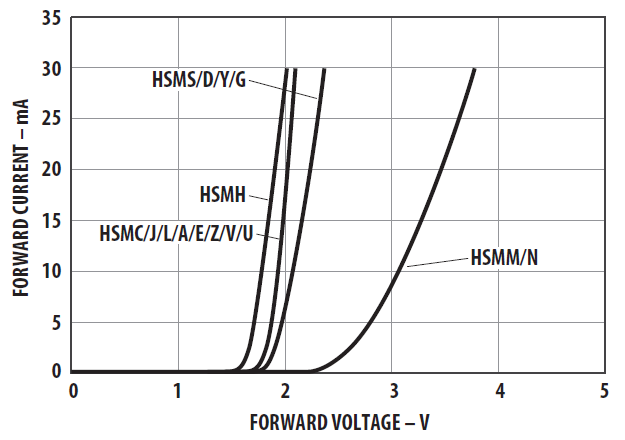
\includegraphics[width=0.8\textwidth]{Kennlinien_LED_SMD.png}
 \caption{Kennlinien forward current vs. forward voltage der unterschiedlichen SMD-LED's \cite{LED}}
 \label{fig:Widerstände}
  \end{center}
\end{figure}
Anhand dem Bestand im Labor der OTH, fiel die Entscheidung auf die Widerstandsreihe R0603. Auch die Auswahl der LED's erfolgte nach diesem Kriterium für die HSMx-A100-Reihe von Avago. 

Hierbei ergeben sich aus dem Datenblatt unterschiedliche forward voltage für die jeweilige Leuchtfarbe. Die Berechnung der Widerstände erfolge allerdings immer nach demselben Prinzip. 
Dabei wurde zunächst die jeweilige forward voltage ermittelt und anschließend mit der Batterieversorgung von 3.3 V und einem gewünschten Strom von 10 mA der resultierende Widerstand berechnet. 

Die Festlegung auf 10 mA erfolgte vor allem aus Erfahrung und aus Gründen des Stromverbrauchs. Der normale Betrieb liegt bei 20 mA, dies ist allerdings recht hell und bei einer meist dunklen Party erschienen somit auch 10 mA ausreichend, was günstiger für den Stromverbrauch ist.\\

\newpage

Bei der roten LED1 handelt es sich um eine HSMS-A100-J00J1. Mit dieser Information lässt sich die entsprechende Kennlinie und damit die resultierende forward voltage von 2.1 V ermitteln.
Die folgende Berechnung für den Vorwiderstand ist also:

$$ R1 = (3.3 - 2.1)V / 10mA = 120 \Omega$$

Als letztes muss noch überprüft werden, ob dieser Wert auch innerhalb der R0603-Reihe vorhanden ist oder ob ein naheliegender Wert gewählt werden muss. Da allerdings 120 $\Omega$ vorkommen, kann der exakte Wert für die Schaltung verwendet werden. \\

Die selben Schritte erfolgen nun auch für die weiteren LED's, wodurch sich für die gelbe LED2 (HSMY-A100-J00J1) dieselbe forward voltage ergibt. Dadurch ist nun die Berechnung gleich der Rechnung für die rote LED:

$$ R2 = (3.3 - 2.1)V / 10mA = 120 \Omega$$

Und auch hier kann direkt der richtige Wert aus der Reihe genommen werden.\\ 

Zum Schluss noch zur grünen LED3, dem Bauteil HSME-A100-L01J1. Hier lässt sich eine forward voltage von 1.8 V aus dem Diagramm ablesen. 
Dadurch ergibt sich für den Widerstand:

$$ R3 = (3.3 - 1.8)V / 10mA = 150 \Omega$$

Nach der Reihe R0603 ergibt das auch einen Widerstand von 150 $\Omega$.

\newpage
\section{Kapazitiver Sensor}
Als nächstes wird der Kapazitive Sensor erläutert, der für die Weiterschaltung der LED's zuständig ist. Grundsätzlich ist zu sagen, dass alle Kapazitiven Sensoren auf einem RC-Oszillator basieren. Kommt es zu einer Berührung oder Näherung durch beispielsweise einem Finger so wird die Kapazität und somit die Lade- und Entladezeit des Oszillators erhöht. Es gibt verschiedene Möglichkeiten dies zu detektieren. Nachfolgend sind einige davon aufgelistet, die für das Projekt in Betracht gezogen wurden.

\subsection{Verschiedene Varianten von Kapazitiven Sensoren}
\label{VerschiedeneKapSenVar}

\subsubsection{Komparator}
Zuerst wird die Komparator-Methode erklärt. Hierbei wird ein Dreieck-Signal an einem RC-Ladeglied angelegt. Durch das RC-Glied wird das Signal abgerundet ähnlich wie in Abbildung \ref{fig:Tiefpass} zu sehen. Dieses Signal und eine feste Gleichspannung wird nun an einen Komparator angelegt. Jedes Mal wenn der Komparator umschaltet wird die vergangene Zeit gemessen. Gibt es eine Berührung so wird das Dreieck-Signal stärker abgerundet und somit verändert sich auch die Zeit die der Komparator zum Umschalten braucht. Durch dieses Prinzip können auch relativ elegant Timer und Interrupts verwendet werden. 
\begin{figure}[!hbpt]
 \begin{center} 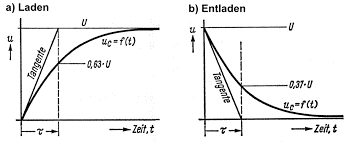
\includegraphics[width=1\textwidth]{RCTiefpass.png}
 \caption{RC-Tiefpass}
 \label{fig:Tiefpass \ref{RCTiefpass}}
  \end{center}
\end{figure}

\subsubsection{ADC}
Als nächstes wird die Variante erklärt, die einen Analog-Digital-Wandler verwendet. Hierbei wird ein RC-Ladeglied auf den logischen High-Pegel aufgeladen und nach einer festen Zeit mithilfe des ADC gemessen. Die gemessene Spannung ist dabei abhängig von der Kapazität des Ladeglieds. Ist die Kapazität nicht erhöht, also keine Berührung oder Näherung von zum Beispiel einem Finger, so entlädt sich die Spannung schneller. Gibt es aber eine Berührung oder Näherung so ist die Kapazität höher und die Entladekonstante des RC-Glieds größer, was zu einem zeitlich längeren Spannungsabfall führt. Zusammengefasst ist also die Spannung, die der ADC misst größer wenn eine Berührung oder Näherung statt gefunden hat. 

\subsubsection{Sende- und Empfangspins}
Die dritte Variante ist jeweils einen Sende- und Empfangspin zu benutzen. Dabei wird ein sehr hochohmiger Widerstand zwischen zwei Pins gesetzt, der mit der Kapazität des Receivepins ein RC-Tiefpass realisiert. Verändert man nun den Logik-Pegel am Sendpin so dauert es, wegen dem Tiefpass, eine kurze Zeit bis diese Änderung am Receivepin ankommt. Diese Zeit ist messbar und je nach Kapazität unterschiedlich. Die unterschiedliche Kapazität ist auf ein Metallstück oder Folie, welches am Receivepin befestigt ist, zurückzuführen. Berührt man diese Folie so wird, wie bei der ADC-Variante, die Ladekonstante erhöht und es dauert länger bis eine Änderung des Sendpins am Receivepin erkannt wird. Dieser Aufbau ist im Abbildung \ref{fig:KapSensor} veranschaulicht.

\begin{figure}[!hbpt]
 \begin{center} 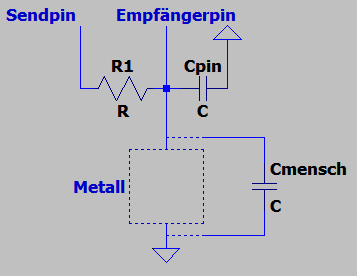
\includegraphics[width=0.6\textwidth]{KapazitiverSensor.png}
 \caption{Funktionsweise des Kapazitiven Sensors}
 \label{fig:KapSensor}
  \end{center}
\end{figure}

\subsection{Bewertung}
\label{Bewertung}
Als nächstes werden die Varianten aus \ref{VerschiedeneKapSenVar} bewertet. Die erste Lösung ist hier sehr umständlich umzusetzen, da der Mikrocontroller STM32G0316J6M6 keinen Komparator besitzt. Deswegen wurde diese Variante nicht verwendet.

Die ADC-Methode hat den großen Vorteil, dass sie nur ein Pin benötigt. Sie braucht jedoch eine zusätzliche Kapazität, was Platz verbraucht und Kosten verursacht. Zudem besitzt der Mikrocontroller nur einen Analog-Digital-Wandler, welcher gegebenenfalls anderweitig für einen Sensor hätte verwendet werden können. 
Die letzte Variante ist auch die Einfachste. Sie braucht nur einen Widerstand und hat keine besonderen Anforderungen an die Hardware des Mikrocontrollers. Der größte Nachteil ist hier allerdings, dass zwei Pins benötigt werden. Pins können aber trotzdem mehrfach verwendet werden, was in \ref{Energie} näher erklärt wird. Letztendlich wurde sich für die Sende- und Empfangsmethode entschieden.


\subsection{Umsetzung}
Dieser Abschnitt beinhaltet die Umsetzung der Variante, welche unter \ref{Bewertung} ausgewählt wurde. Grundsätzlich ist zu sagen, das der Sensor in der jetzigen Form sehr ungenau und unzuverlässig ist. Um dies zu ändern und eine auswertbare Messung zu erhalten muss der Vorgang mehrfach hintereinander durchgeführt werden, damit eventuelle Fehlerquellen ermittelt und behoben werden können. 

Ein großes Problem ist zudem, dass der Receivepin nach einer einzelnen Messung nicht auf einen vollen HIGH- bzw. LOW-Pegel aufgeladen wird, was schlecht für die nächste Messung wäre.

Der Receivepin meldet also einen HIGH-Pegel schon bei beispielsweise 1.8 V, was das Ende der Messung bedeuten würde, obwohl für den nächsten Zyklus 3.3 V an diesem Pin benötigt werden. Deswegen wird der Pin danach als Output deklariert und der entsprechende Pegel angelegt bis dort die 3.3 V bzw. 0 V anliegen. Zusätzlich werden Pullup- und Pulldownwiderstände genutzt um diesen Prozess zu beschleunigen. 

Zu Beginn des Projektes wurde der Kapazitive Sensor mit einem Metallteil, welches mit einem Kabel verbunden ist, ausgetestet, was gut funktioniert hat. Nur für eine kompakten und vor allem einfachen Aufbau ist dies groß bzw. zu kompliziert zu erstellen. Deswegen wurde auf ein bereits bestehendes Metall zurückgegriffen nämlich das Kupfer der Platine. Es wurden vier kreisförmige Flächen angelegt, die den Designrules \ref{Guidelines}von STM entsprechen. Dadurch könnte auch ohne externes Metallteil eine Berührung erkannt werden.

Ein weiterer wichtiger Punkt ist die Größe des Widerstandes, da dieser der Sensitivität des Sensors entspricht. Bei einem Widerstand von beispielsweise 1 MOhm wird nur ein direkter Kontakt erkannt. Wird dieser erhöht so kann auch eine Näherung oder Kontakt über eine kurze Luftlinie bzw. durch ein anderes Material gemessen werden. Dieses Konzept wurde auch bei diesem Projekt umgesetzt, da auch durch das Gehäuse eine Berührung erkannt werden soll. Deswegen wurde ein 4,7 MOhm Widerstand verwendet. Außerdem wurde das Gehäuse so angepasst, dass die herausstehenden Zylinder die Kupferflächen des Sensors und das Gehäuse direkt verbinden. Ein großer Luftspalt zwischen diesen beiden Komponenten würde es hier sehr schwierig machen einen Kontakt zu unterscheiden. Aus dem selben Grund wurde auch noch Sekundenkleber verwendet. 

Bei der Pinbelegung wurden zuerst Pin 4 und 5 gewählt. Der Grund dafür war das die Pins des Mikrocontrollesr, welche für die Single-Wire-Debug-Schnittstelle zuständig sind unbenutzt bleiben sollten um das debuggen zu ermöglichen. Das Problem hieran war, dass der Pin 4 der Reset-Pin ist und teilweise beim testen eine Stuck-at-1-Fehler aufwies. Dies ließ den Mikrocontroller im Reset-Zustand verweilen, was den Ablauf des Programmes und das Debuggen verhinderte. Deswegen wurde der Kapazitive Sensor auf Pin 5 und 6 gelegt.
 
\subsection{Störquellen und Probleme}
Schlussendlich muss leider gesagt werden, dass einige Probleme nicht perfekt gelöst werden konnten. Einer ist das weiter schalten des Zustandes ohne Masseverbindung. Der Grund dafür ist, dass überall andere elektromagnetische Begebenheiten herrschen, die eine Masseverbindung abfangen würde. Dadurch ist auch die Zeit, die der Empfangspin zum erkennen benötigt und damit der Schwellenwert für die Berührungsentscheidung anders. Deswegen ist der kapazitive Sensor ohne Masseverbindung relativ unzuverlässlich. Die Lösung dafür wäre ein dynamischer Schwellenwert. Dies würde aber vom Aufwand her die Vorgaben weit überschreiten. 

Außerdem wurde festgestellt, dass sich das System selbst beeinflussen kann. So ist es möglich bei eingeschalteter Gelben-Led und Anwesenheit eines Gehäuses ein Sensor-Timeout hervorzurufen. Ein Sensor-Timeout heißt hier, dass der Empfangspin des Sensors sich zu langsam oder gar nicht ändert. Dieses Problem konnte nicht näher betrachtet werden, da es keine kurzfristige Möglichkeit gab ein Oszilloskop anzuschließen.



\newpage
\section{Energiesparmodus}
\label{Energie}
Als nächstes sollen die verschiedenen Möglichkeiten Strom zu sparen betrachtet werden. Der simpelste Ansatz wäre hier ein PWM-Signal für die LED's zu benutzen, um so Strom einzusparen. Diese Variante ist bei der verwendeten LED-Schaltung aber nicht ganz einfach, da man Extra-Pins für die Versorgung bräuchte. 

Eine weitere Möglichkeit ist der LowPowerMode des Mikrocontrollers. In diesem Modus wird wesentlich weniger Strom verbraucht als normal und es gibt keine Änderung der Output-Pins. Dadurch kann auch ein Lock-Mechanismus für den Kapazitiven Sensor realisiert werden. Der LED-Zustand kann also nicht verändert oder weiter geschaltet werden. Dies ist nützlich um eine versehentliche Änderung, durch Berühren oder Störungen, zu verhindern. Um in diesem Zustand hinein und wieder herauszukommen wird ein Schalter benutzt der den ReceivePin des Kapazitiven Sensor also Pin 5 benutzt. Wird dieser geschaltet so entsteht eine Verbindung zwischen Pin 5 und Vcc und der Code geht in den Energiesparmodus. Generell werden durch diese Anordnung keine Extra-Pins benötigt. Ein Grund dafür ist, das die Verbindung zu 3.3 V zyklisch abgefragt wird. 

Der Stromverbrauch der einzelnen Zustände wurde letztendlich gemessen und in Tabelle \ref{tab:ADEinton} dargestellt.

\begin{table}[h]
\begin{center}
\rowcolors{3}{lightgray}{white}
\begin{tabularx}{\columnwidth}{XX}
Normalbetrieb & 7,6mA \\ 
Energiesparmodus mit LED & 6,2mA\\
Energiesparmodus ohne LED & 0,24mA
\label{tab:ADEinton}
\end{tabularx}
\end{center}
\caption{Stromverbrauch unterschiedlicher Modi}
\end{table}





\newpage
\section{Schaltplan und Layout}

Die Gestaltung der Platine setzt sich zusammen aus der Erstellung des Schaltplans, nach den zuvor ermittelten Funktionen. Das Layout wird anhand des Schaltplans erstellt und mit den gegebenen Vorgaben für die äußere Erscheinung der Ampel. Beides erfolgt mit dem Programm KiCAD, für das im Vorfeld ein Einführungskurs an der OTH besucht wurde.

\subsection{Schaltplan}

Als erstes wird der Schaltplan in 6 verschiedene Teile unterteilt um das Folgende übersichtlicher zu gestalten. Diese Teile sind: Batterieversorgung, kapazitiver Sensor, LED-Schaltung, Energiesparmodus-Schalter, Connector, Mikrocontroller


\paragraph{Batterieversorgung} $~$ \\

Da es sich um ein möglichst minimalistisches System handelt, ist ein Knopfzellenbetrieb notwendig. Eine passende Batteriegröße dafür ist 3032 und es gibt unterschiedliche Batteriehalter für eine solche Batterie. Aus diesem Grund wurde der Batteriehalter nach einem passenden Package für KiCAD ausgewählt, da das für die Layouterstellung einfacher ist. Die Wahl viel somit auf ein Modell von Renata. 

Der Batteriehalter befindet sich in der linken oberen Ecke von Abbildung \ref{fig:Schaltplan}. Das Package war von den +/- Belegungen vertauscht, was allerdings später beim Layout entdeckt wurde.

\paragraph{kapazitiver Sensor} $~$ \\

Der kapazitiver Sensor (Abbildung \ref{fig:Schaltplan} oben mittig) wurde wie nach Kapitel 4.1.3 mit einem Sende- und Empfangspin realisiert. Sie sind an Pin 5 und 6 des Mikrocontrollers angeschlossen. Als nächstes wurde ein Jumper eingesetzt um die Möglichkeit offen zu halten den kapazitiven Sensor entweder mit Pads oder einem Connector zu verbinden. Der Connector war als gesicherte Methode gedacht, bei der eine Metallplatte angeschlossen wird als Sensor. Dies war später allerdings nicht notwendig, da der Sensor mit den Pads funktioniert hat und deshalb wurde auch ein Widerstand von 4.7 MOhm ausgewählt, der dazu passt.

\newpage

\paragraph{LED-Schaltung} $~$ \\

Die LED-Schaltung (Abbildung \ref{fig:Schaltplan} oben rechts) ist an dieser Stelle recht simpel zu erklären, da auf die Hintergründe ihrer Entstehung bereits in Kapitel 3.2 eingegangen wurde. 
Die Pins des Microcontrollers wurden danach ausgesucht, dass es sich dabei nicht um Debug-Pins handelt und aus diesem Grund wurden Pin 5 und 6 gewählt.

\paragraph{Energiesparmodus-Schalter} $~$ \\

Es wurde ein Schalter (Abbildung \ref{fig:Schaltplan} unten rechts) ohne Durchkontaktierung ausgewählt (JS102011SAQN von C \& K Components). Der Schalter soll dabei die funktionierende Schaltung nicht beeinträchtigen, aber den Energiesparmodus aktivieren. Aus diesem Grund ist der dritte Kontakt des Schalters nicht angeschlossen und ermöglicht den normalen Betrieb. Wenn der Schalter \glqq aktiviert\grqq{} ist, ist er über Pin 5 mit dem Mikrocontroller verbunden und dadurch wird der Energiesparmodus eingeschaltet. 


\paragraph{Connector} $~$ \\

Der Connector (Abbildung \ref{fig:Schaltplan} unten mittig) ermöglicht lediglich den Mikrocontroller mit dem entsprechenden Code zu bespielen. Es ist die einfachste Möglichkeit den Mikrocontroller mit dem USB-Stick ST-Link V2 zu programmieren. Die minimale Anzahl an Pins ist hierbei 4 für Ground, Reset, SWCLK und SWDIO.

\paragraph{Mikrocontroller} $~$ \\

Der Mikrocontroller (Abbildung \ref{fig:Schaltplan} mittig) ist zum einen mit Ground und 3.3 V von der Batterie verbunden. Eine weitere Belegung von Pin 4 und 8 führte zu Fehlern, aus diesem Grund werden nur die anderen Pins überbelegt. Dies war notwendig, da der Microcontroller lediglich 8 Pins zur Verfügung stellt und bereits 4 wegfallen. Die übrig gebliebenen 4 müssen also 6 Funktionen ausführen. Das Package für den Mikrocontroller konnte für KiCAD heruntergeladen werden.

\begin{figure}[!hbpt]
 \begin{center} 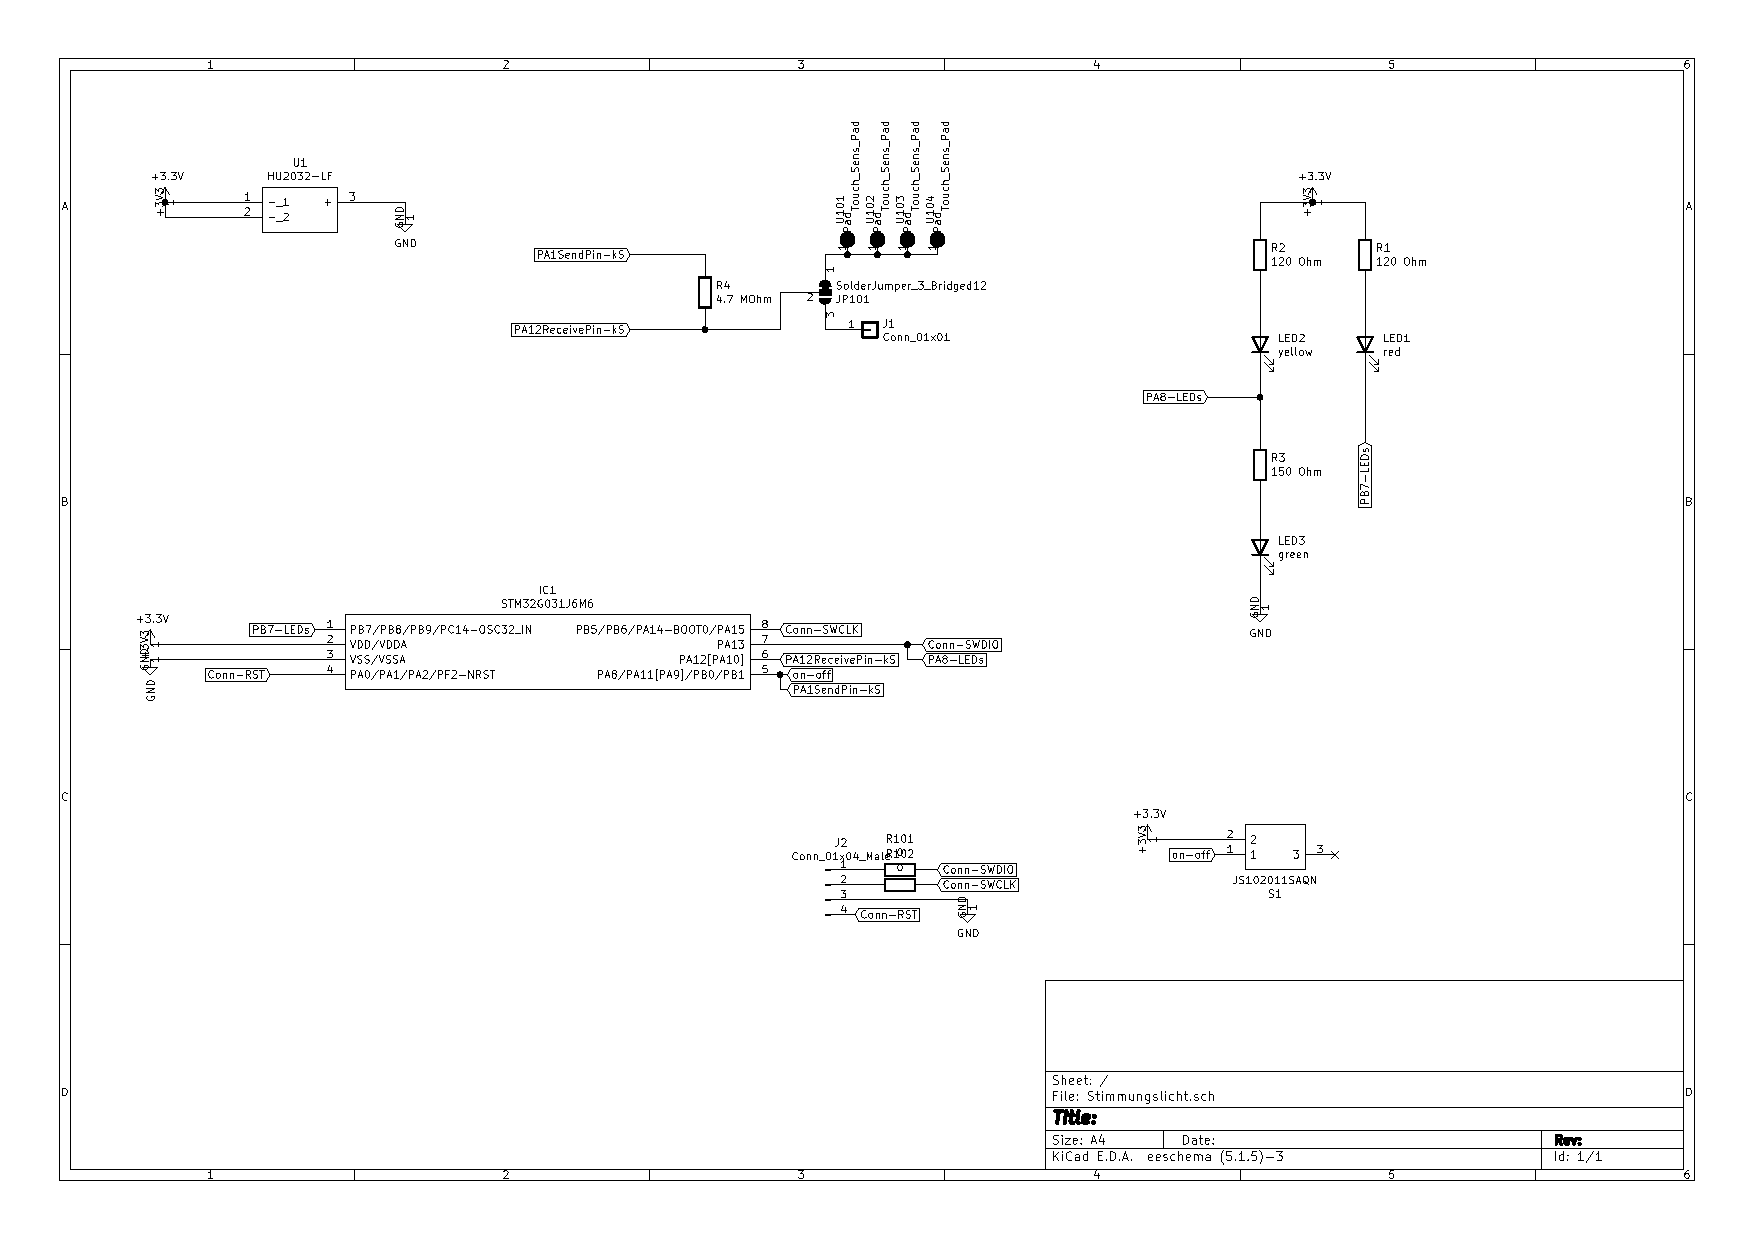
\includegraphics[width=1.4\textwidth,angle=90]{Schaltplan.pdf}
 \caption{Schaltplan}
 \label{fig:Schaltplan}
  \end{center}
\end{figure}

\newpage

\subsection{Layout}

Das Layout wird anhand des Schaltplans mit KiCAD erstellt, dabei werden die entsprechenden Bauteile ausgewählt und dann in PCB überliefert. Als erstes wird der Umriss der Platine als Kreis erstellt mit einem Durchmesser von unter 4 cm. Es müssen auch die Leitungsparameter festgelegt werden, die so ausgewählt wurden, dass eine Fräsung bei der OTH möglich war. Also breiter als normalerweise bei dem vorhandenen Strom notwendig gewesen wäre. Nun gilt es die Bauteile zu platzieren und die Leitungen zu ziehen. Die im Folgenden beschriebenen Teile sind in Abbildung \ref{fig:Front} für den Front-Layer und in Abbildung \ref{fig:Back} für den Back-Layer ersichtlich.

\paragraph{Batterieversorgung} $~$ \\

Es ist wenig Platz auf der Platine vorhanden, deshalb ist der Batteriehalter auf der Rückseite platziert. Man kann seine Durchkontaktierungen oben doppelt und unten als einen Kontakt in den Abbildungen \ref{fig:Front} und \ref{fig:Back} erkennen. 

\paragraph{LED-Schaltung} $~$ \\

Die LED's wurden als nächstes mittig platziert, da sie die Ampelschaltung anzeigen. Alle anderen Bauteile werden um sie herum platziert.

\paragraph{Energiesparmodus-Schalter} $~$ \\

Der Schalter für den Energiesparmodus ist seitlich direkt am Rand der Platine platziert, damit er von außen bedient werden kann. 

\paragraph{Mikrocontroller} $~$ \\

Da die meisten Leitungen zum Mikrocontroller führen ist es sinnvoll diesen möglichst mittig zu platzieren um lange Leitungen zu vermeiden. In diesem Fall bedeutet das allerdings nur so mittig wie möglich, da sich die LEDs bereits dort aus optischen Gründen befinden. 

\paragraph{Connector} $~$ \\

Der Connector befindet sich möglichst neben dem Mikrocontroller damit die Leitungen nicht zu lang werden.

\paragraph{kapazitiver Sensor} $~$ \\

Der kapazitive Sensor erhielt sozusagen den übrig gebliebenen Platz. Da die Sensorflächen äußerst groß sind und nicht zu nah an den Connectoren, aufgrund von Störungen, platziert werden sollten, ist der einzige Platz oberhalb der LED's. 

Dies ist nur die erste Hälfte des Sensors. Der Connector muss möglichst weit am Rand sein, da der Draht, der nach Außen zu einer Metallplatte führt nicht unnötig lang sein soll. 

Dadurch ist es schwierig die Sensorpads an den Mikrocontroller anzuschließen, da sie weit voneinander entfernt sind. So wurde auf den Back-Layer, wie in Abbildung \ref{fig:Back} zu erkennen, für die Leitungen zurückgegriffen. Den Pads wurde außerdem eine Durchkontaktierung hinzugefügt.\\


Um Überschneidungen in den Leitungen zu vermeiden wurden noch zwei zusätzliche Widerstände mit 0 Ohm hinzugefügt. Alle Leitungen laufen über das Front-Layer wie in Abbildung \ref{fig:Front} zu erkennen ist. Lediglich der kapazitive Sensor wurde rückseitig (Abbildung \ref{fig:Back}) verdrahtet. 

Im letzten Schritt wird die Platine als Massefläche gesetzt um Störungen zu vermeiden. Das war aufgrund der runden Form nur durch das Nachzeichnen dieser Form in KiCAD möglich. 

\begin{figure}[!hbpt]
 \begin{center}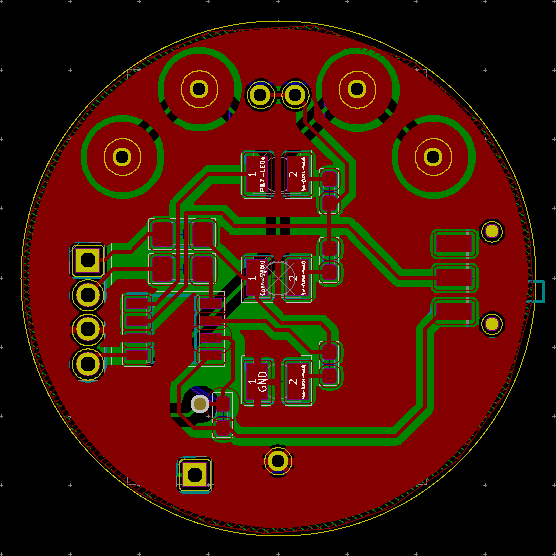
\includegraphics[width=0.6\textwidth]{Layout_Front.png}
 \caption{Layout - Front Layer}
 \label{fig:Front}
 \end{center}
\end{figure}

\begin{figure}[!hbpt]
 \begin{center} 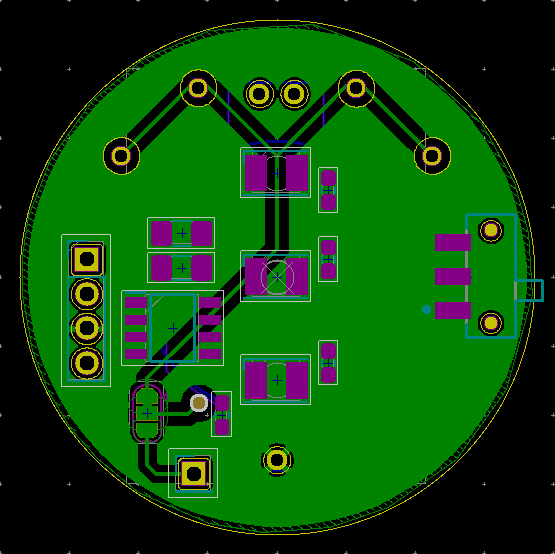
\includegraphics[width=0.6\textwidth]{Layout_Back.png}
 \caption{Layout - Back Layer}
 \label{fig:Back}
  \end{center}
\end{figure}

\newpage

\section{Gehäuse}
Das Gehäuse besteht aus einem Grundbehältnis und einem Deckel, welche zunächst in SolidWorks entworfen und dann mit Hilfe eines 3D-Druckers gedruckt wurden. Dabei hat sich das Gehäuse im Laufe der Projekts schrittweise weiter entwickelt. Der Deckel und der Behälter wurden in getrennten Projekten entworfen. 

Die zugehörigen Abbildungen \ref{fig:Grundbe} und \ref{fig:Deckel} wurden mit Solid Edge erstellt und zeigen die Bemaßungen des im Folgenden beschriebenen Gehäuses.

\begin{figure}[!hbpt]
 \begin{center} 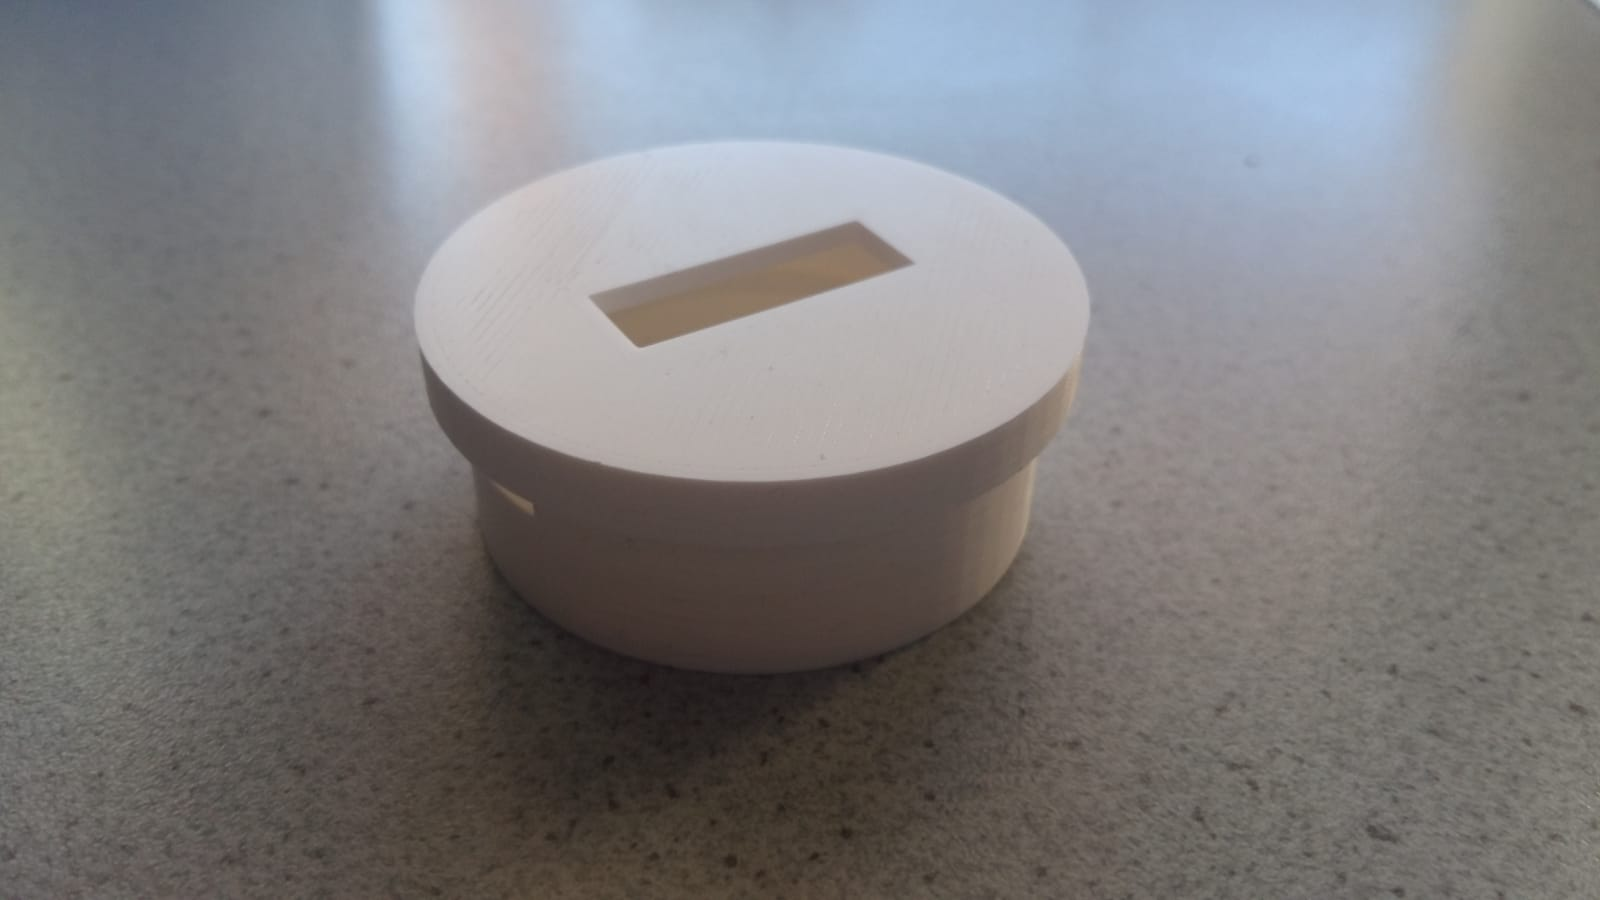
\includegraphics[width=1\textwidth]{Gehaeuse_Stimmungslich.jpg}
 \caption{3D gedrucktes Gehäuse}
 \label{fig:Register}
  \end{center}
\end{figure}

\subsection{Grundbehältnis} $~$ \\
Das Grundbehältnis wurde im ersten Schritt einfach als eine Skizze gezeichnet, die anschließend als Rotation 360° ausgeprägt wird. So entsteht das Grundgerüst eines nach oben geöffneten Hohlzylinders, der eine exakte Passung für die runde Platine darstellt. Es wurde eine Stärke von 2 mm für die Außenwand gewählt. 

Als nächstes ist es wichtig noch den Schalter für den Energiesparmodus von außen bedienen zu können. Dafür ist eine Aussparung im Gehäuse notwendig. Am einfachsten ist es die Aussparung bis zum oberen Rand durchzuführen. Die Aussparung besitzt eine Breite von 11 mm, wodurch ein 1 mm Rand auf beiden Seiten entsteht, da der Schalter eine Breite von 9 mm nach Datenblatt hat. 

Die Aussparung muss allerdings an der richtigen Höhe und Stelle für den Schalter platziert werden. Um das zu ermöglichen braucht die Platine eine Halterung, die sie im richtigen Abstand zur Aussparung hält. Die einfachste Lösung hierfür ist eine Art Ring, der innen im Hohlzylinder angebracht wird. Dafür wurde die anfängliche Skizze des Hohlzylinders angepasst mit einer 1.5 mm in den Zylinder hinein ragenden Kante. Diese Kante ist auf der richtigen Höhe, damit darunter noch der Batteriehalter Platz hat. Die Aussparung für den Schalter geht dann bis knapp über dieser Kante.

Um nun auch den Schalter an der richtigen Stelle zu haben ist es nötig, dass die Platine sich nicht verdreht. Das typische Mittel dafür ist eine kleine Nut, die eine Verdrehung verhindert. Somit wurde eine kleine Nut direkt oberhalb der Kante eingefügt, die so auf der Höhe der Platine liegt. Die Nut ist an der Stelle platziert, wo am meisten Platz auf der Platine vorhanden ist. Also am unteren Rand der Platine, unterhalb der Ground-Verbindung des Batteriehalters also 90° versetzt zur Aussparung des Schalters. 

Nun ist die grundlegende Form des Behälters abgeschlossen. 

Als letzte Verbesserung haben wir entschieden, die Connector-Pins nicht mehr nach oben anzulöten, sondern nach unten. Dadurch wird der Behälter in seiner Höhe reduziert und so handlicher und besser zu befestigen. 

\subsection{Deckel} $~$ \\

Das Grundgerüst des Deckels ist mit dem Grundbehältnis identisch. Auch der Deckel besteht aus einem einseitig geöffneten Hohlzylinder. Die Stärke des Zylinders beträgt dabei, wie zuvor, 2 mm. Zuerst muss hierfür eine Skizze erstellt werden, die anschließend mit einer Rotation 360° 3D-ausgeprägt wird. Die Höhe des Zylinders ist dabei auf die Höhe des Energiesparschalters angepasst. 

Im nächsten Schritt wurde der lineare Ausschnitt erstellt, der alle LED's umfasst und somit die Sicht auf die Ampel ermöglicht. Der Ausschnitt ist zentriert und etwas größer als der Abstand der LED's. 

In der ersten Version des Gehäuses war hiermit der Deckel fertig. Es folgte jedoch eine erneute Überarbeitung, weil ein direkter Kontakt zwischen Sensorflächen und dem Gehäuse für die Funktionalität des kapazitiven Sensors notwendig war. Dafür wurden kleine Vollzylinder erstellt, die exakt an derselben Stelle positioniert sind und denselben Durchmesser haben, wie die Sensorflächen. Die Höhe der Zylinder ist dabei so groß, dass wenn der Deckel sich auf dem Grundbehältnis befindet sie genau auf der Platine aufliegen.  

\subsection{Befestigung} $~$ \\

Die Befestigung für die Ampelschaltung soll möglichst einfach und leicht reproduzierbar sein. Deshalb erschien eine Broschenadel (Abbildung \ref{fig:Nadel})am einfachsten. Diese sind gut für die Befestigung auf Höhe des Brustbereichs und können in passenden Größen bestellt werden mit Klebesockel. 

\begin{figure}[!hbpt]
 \begin{center} 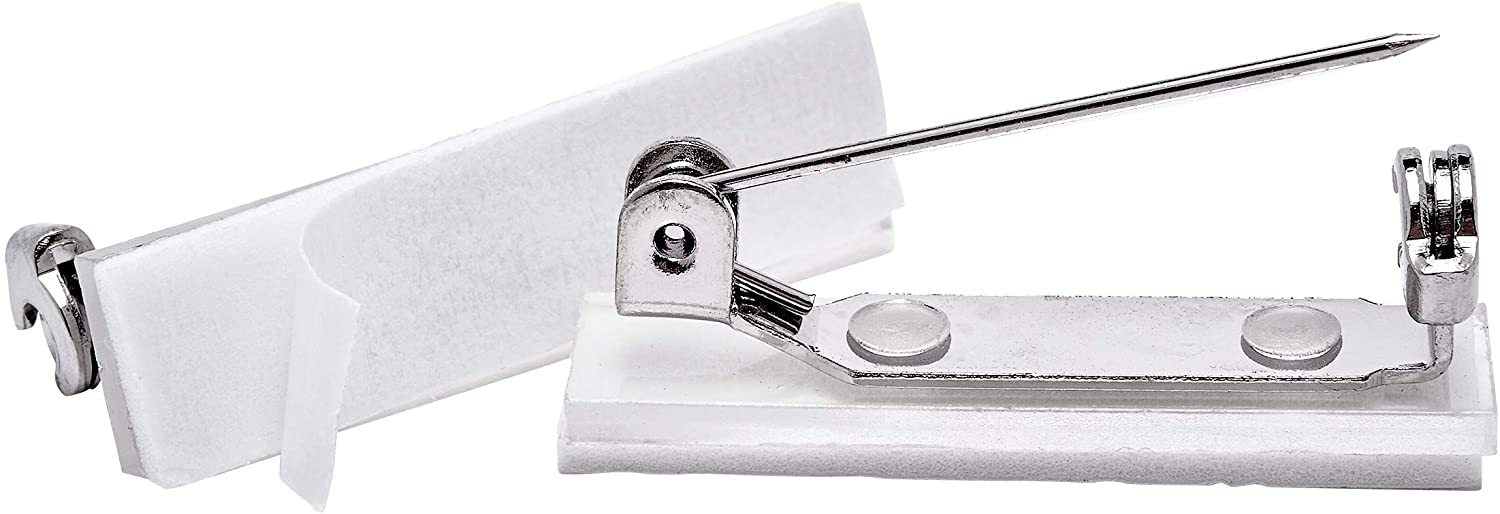
\includegraphics[width=0.8\textwidth]{Broschenadel.jpg}
 \caption{bestellte Broschenadel zur Befestigung \cite{Broschenadel}}
 \label{fig:Nadel}
  \end{center}
\end{figure}


\begin{figure}[!hbpt]
 \begin{center} 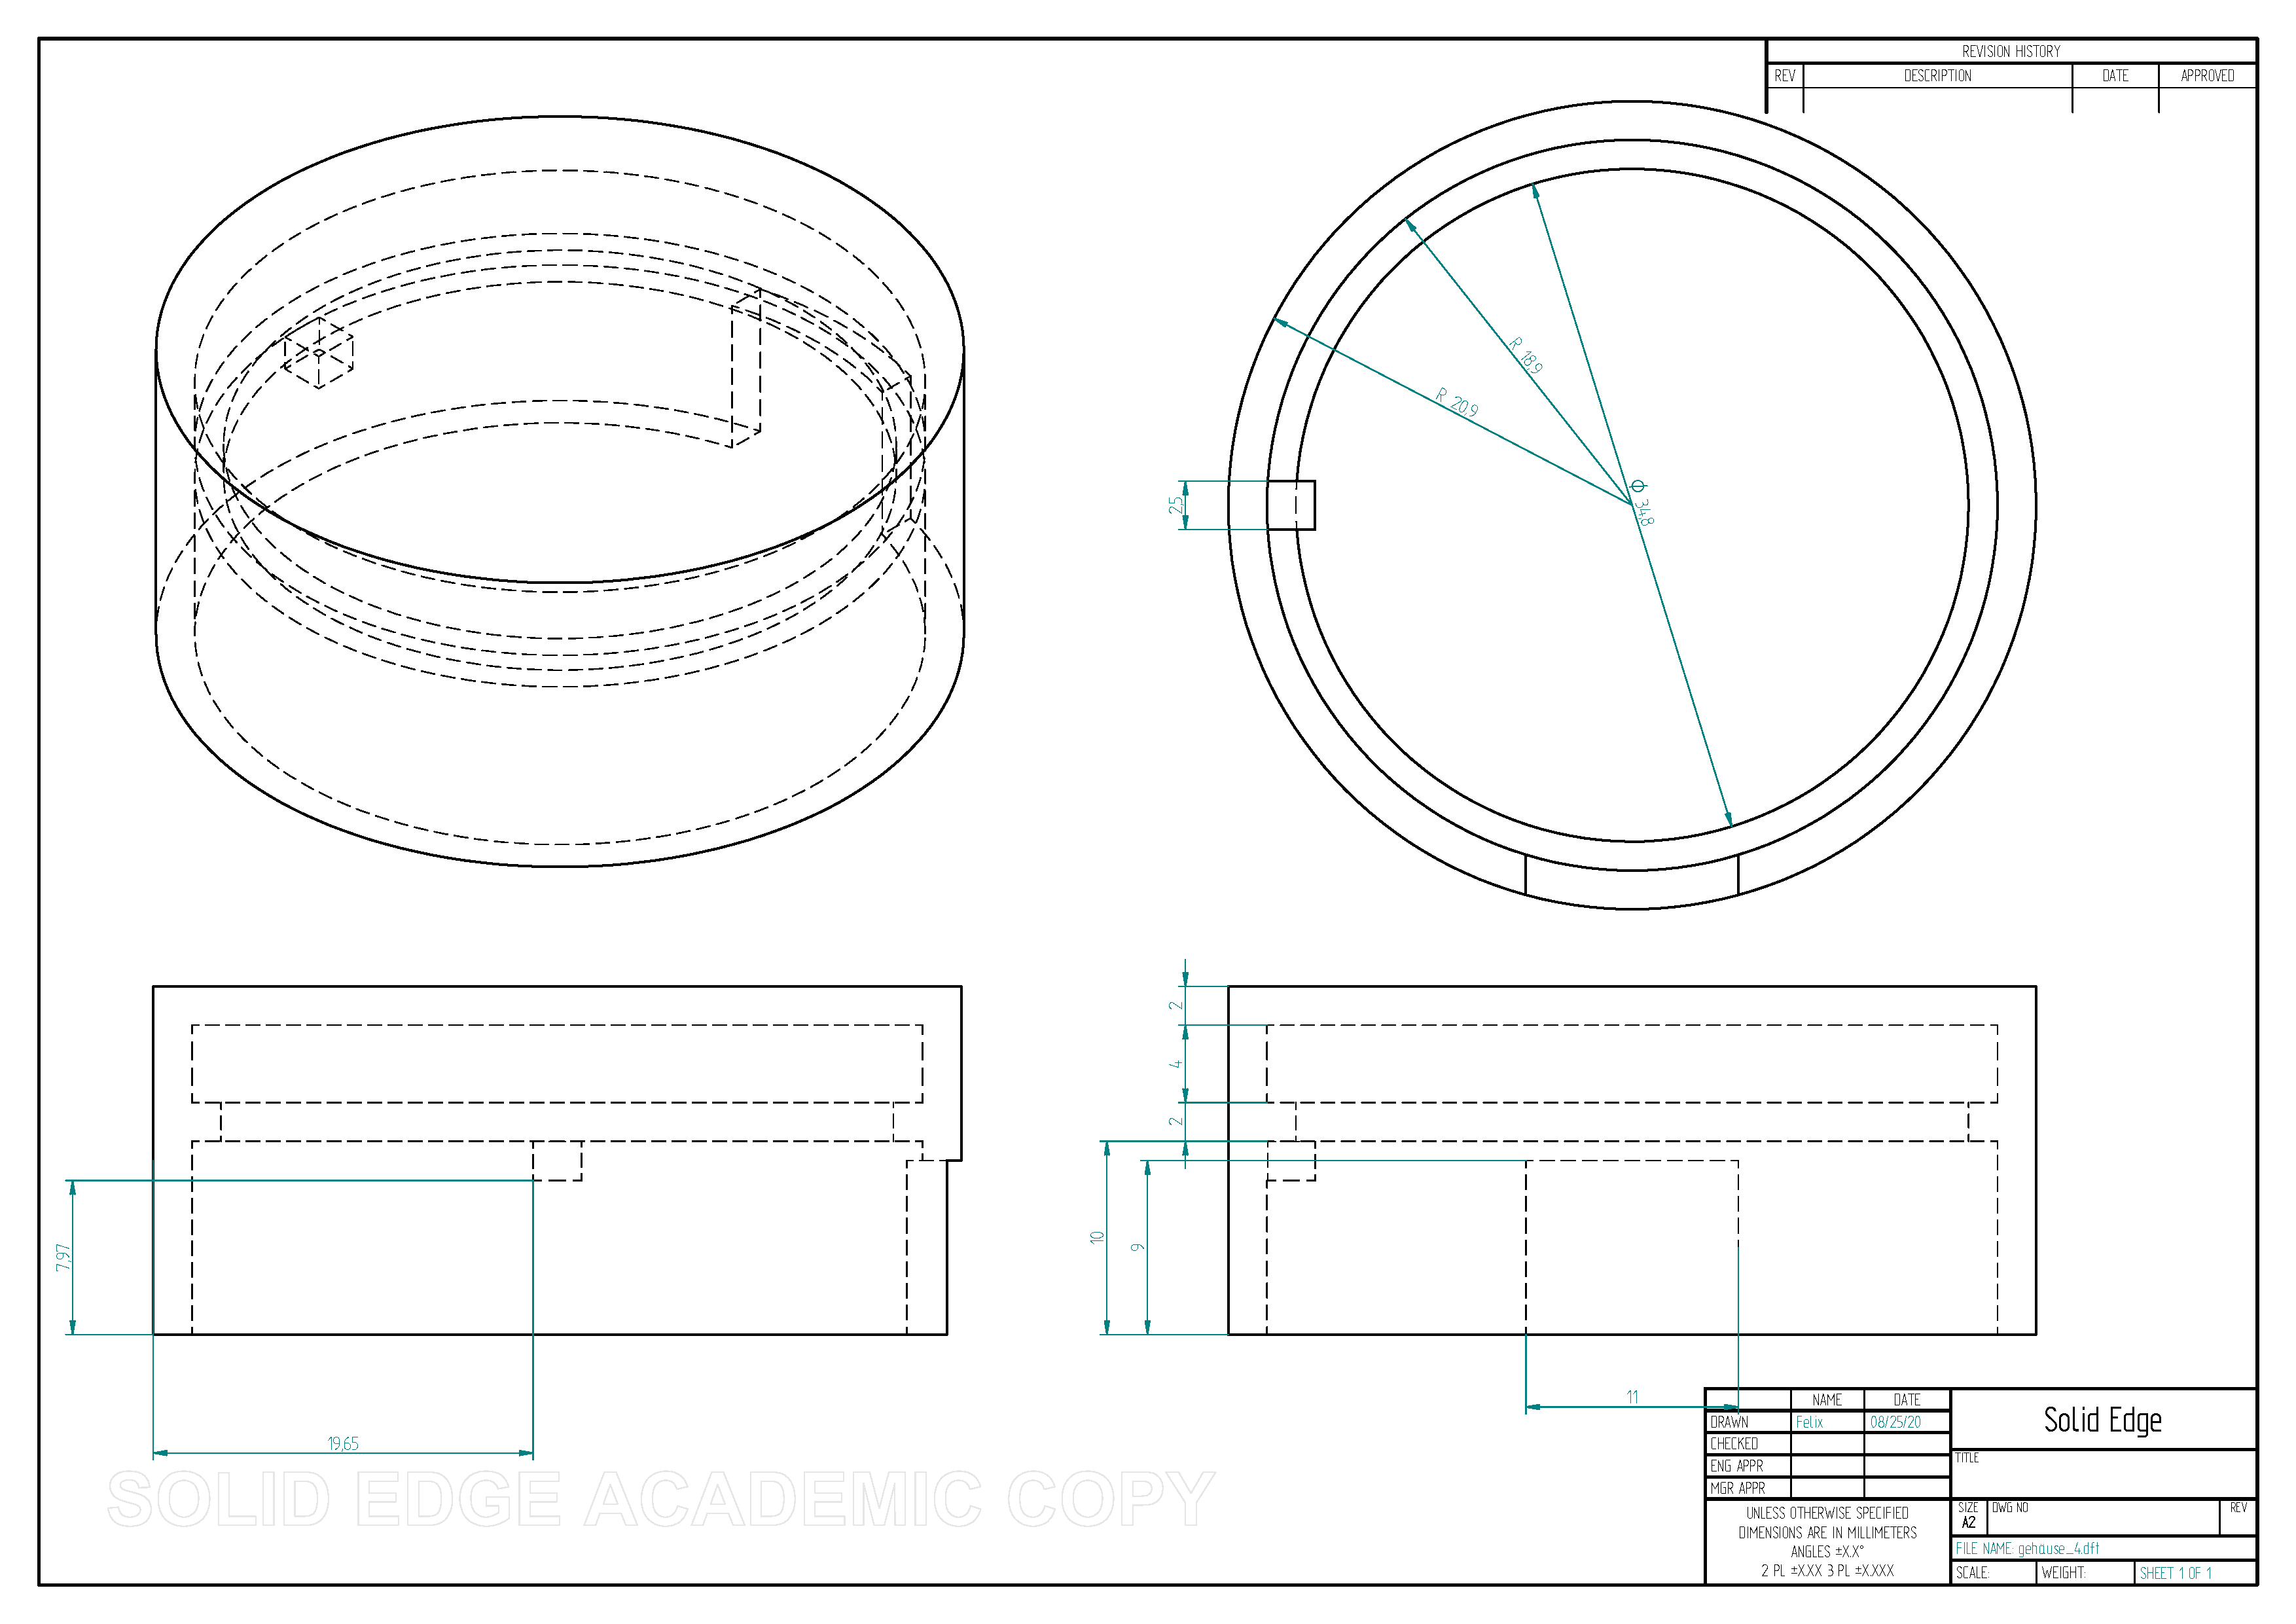
\includegraphics[width=1.4\textwidth,angle=-90]{gehauuse_4.pdf}
 \caption{Grundbehältnis des Gehäuses mit Bemaßungen}
 \label{fig:Grundbe}
  \end{center}
\end{figure}

\begin{figure}[!hbpt]
 \begin{center} \includegraphics[width=1.4\textwidth,angle=-90]{Deckel.pdf}
 \caption{Deckel des Gehäuses mit Bemaßungen}
 \label{fig:Deckel}
  \end{center}
\end{figure}

\newpage

\section{Fazit}

Insgesamt hatte das Projekt sowohl positive als auch negative Seiten.

Was den Mikrocontoller angeht, hat uns dieser viel Einarbeitung und Fehlersuche abverlangt. Dies lag vor allem daran an seiner minimalistischen Auslegung, was bei einem solchen Projekt natürlich seine Berechtigung hat. Allerdings war das auch die größte Hürde mit der es zu kämpfen galt. Eine der größten Verzögerungen entstand durch den stuck-at-1-Fehler, dessen Hintergrund in einer einzigen Zeile im Datenblatt lag, die schwer zu entdecken war.

Die Bauteilauswahl hat insgesamt gut funktioniert und die Arbeit mit den Programmen Solid Works und KiCAD war gemischt. Solid Works hat auch ohne große Einarbeitung sehr intuitiv funktioniert. Bei KiCAD lagen die größeren Probleme, trotz Einführungsveranstaltung. Hierbei funktionierte die Erstellung des Schaltplans recht gut, allerdings gab es etliche Überarbeitungen des Layouts, die viel Zeit in Anspruch genommen haben. Dies lag vor allem in der bisherigen Unerfahrenheit bei der selbstständigen Erstellung einer Platine. Mit der Zeit wurde aber auch dieses besser und es konnte einiges an Erfahrung daraus für folgende Projekte mitgenommen werden. 

Ein weiteres Problem war, dass wegen der Corona-Pandemie lange keine eigenständige Arbeit mit der Platine im Labor möglich war. Da zu Hause das notwendige Equipement zum Löten einer SMD-Schaltung nicht vorhanden war, führte dies zu vielen Verzögerungen. Zum Glück konnte letztendlich doch noch die Platine eigenständig im Labor gelötet werden.

Insgesamt haben wir viele neue Erfahrungen gesammelt durch die Ausdauer, die dieses Projekt erfordertet und das dadurch immer tiefere Eintauchen in die Materie. 






\cleardoublepage
\begin{appendix}
\listoffigures
\listoftables

\cleardoublepage
\begin{thebibliography}{99}
\bibitem{LED} HSMx-A10x-xxxxx, Avago, https://www.infinite-electronic.ru/datasheet/6e-HSMA-A100-Q00H1.pdf.
\bibitem{Broschenadel} 10 Broschennadeln selbstklebend, ca. 30mm , Amazon.
%https://www.amazon.de/gp/product/B008CNY7T2/ref=ppx_yo_dt_b_asin_title_o01_s00?ie=UTF8&psc=1
%\bibitem{Guidelines} dm00445657-getting-started-with-touch-sensing-control-on-stm32-microcontrollers-stmicroelectronics.pdf, https://www.st.com/resource/en/application_note/dm00445657-getting-started-with-touch-sensing-control-on-stm32-microcontrollers-stmicroelectronics.pdf.
%\bibitem{RCTiefpass} einfuehrung_09.pdf,http://www.controllersandpcs.de/lehrarchiv/pdfs/elektronik/einfuehrung_09.pdf.
\end{thebibliography}

\cleardoublepage

\end{appendix}

\end{document}
